\documentclass[11pt]{article}

\usepackage[margin=1in]{geometry}
\usepackage{amsmath,amssymb}
\usepackage{graphicx}
\usepackage{booktabs}
\usepackage{fancyhdr}
\usepackage{titlesec}
\usepackage{caption}
\usepackage{listings}
\usepackage{xcolor}
\usepackage{natbib}
\usepackage[colorlinks=true,linkcolor=blue,citecolor=blue,urlcolor=blue]{hyperref}

% ---- Section numbering with trailing period, e.g. "1. Introduction" ----
\titleformat{\section}{\normalfont\Large\bfseries}{\thesection.}{0.6em}{}
\titleformat{\subsection}{\normalfont\large\bfseries}{\thesubsection.}{0.6em}{}

% ---- Running header: course name (left) / short title (right) ----
\pagestyle{fancy}
\fancyhf{}
\lhead{Independent Study}
\rhead{Markowitz Portfolio Optimization}
\renewcommand{\headrulewidth}{0.4pt}
\cfoot{\thepage}

\fancypagestyle{plain}{%
  \fancyhf{}
  \cfoot{\thepage}
  \renewcommand{\headrulewidth}{0pt}
}

% ---- Code listing style (Appendix B) ----
\lstdefinestyle{python}{
  language=Python,
  basicstyle=\ttfamily\footnotesize,
  keywordstyle=\color{blue!70!black}\bfseries,
  commentstyle=\color{gray},
  stringstyle=\color{green!40!black},
  numbers=left,
  numberstyle=\tiny\color{gray},
  breaklines=true,
  showstringspaces=false,
  frame=single,
  tabsize=4,
}

\title{\textbf{Diversification Under Estimation Risk}\\[4pt]
\large A Markowitz Mean-Variance Analysis of SPY, VXUS, and QTUM}

\author{Marsel Nagimov \\ Independent Study}

\date{September 2026}

\begin{document}

\pagenumbering{arabic}
\maketitle
\thispagestyle{plain}

\begin{abstract}
This project applies the classical Markowitz mean-variance framework to a
three-asset portfolio spanning U.S. equities (SPY), international developed
and emerging-market equities (VXUS), and a thematic quantum-computing
technology fund (QTUM). Using daily adjusted-close prices, we estimate
annualized expected returns and a covariance matrix, then solve for the
global minimum-variance portfolio, the maximum Sharpe ratio (tangency)
portfolio, and the full efficient frontier. The unconstrained optimizer
produces corner solutions: the minimum-variance portfolio allocates entirely
to SPY and VXUS, while the maximum Sharpe ratio portfolio allocates entirely
to QTUM. We argue this is a textbook symptom of estimation risk in
mean-variance optimization rather than a genuine diversification
recommendation, and we compare the optimizer's output against a fixed,
manually diversified 60/20/20 allocation across the same three assets. The
results illustrate a central practical tension in portfolio theory: the
mathematically optimal portfolio is highly sensitive to noisy input
estimates, while a simple diversified heuristic is more robust but
sits strictly inside the efficient frontier.
\end{abstract}

\section{Introduction}

Modern portfolio theory, originating with \citet*{markowitz1952}, formalizes
the intuition that a rational investor should care not only about an
asset's expected return but about how that asset's returns co-move with the
rest of the portfolio. An asset with mediocre expected return can still
improve a portfolio if it is weakly correlated with the investor's existing
holdings, because it reduces total portfolio variance for a given level of
expected return.

This project studies a simple, practically motivated version of that
problem: an investor holding a core U.S. equity position (SPY) considers
adding an international equity fund (VXUS) and a concentrated thematic
technology fund (QTUM) to the portfolio. The central research question is:

\begin{quote}
\textit{Does mean-variance optimization over SPY, VXUS, and QTUM produce a
genuinely diversified portfolio, or does it collapse to a concentrated
corner solution -- and if the latter, is a fixed diversified allocation a
more reasonable choice in practice?}
\end{quote}

To answer this, we estimate the Markowitz efficient frontier from historical
returns, solve for the minimum-variance and maximum-Sharpe portfolios, and
compare both against a simple fixed-weight 60\% SPY / 20\% VXUS / 20\% QTUM
allocation.

\section{Data}

Table~\ref{tab:assets} lists the three exchange-traded funds used in this
analysis.

\begin{table}[h]
\centering
\caption{Asset Universe}
\label{tab:assets}
\begin{tabular}{@{}lll@{}}
\toprule
Asset Class & Ticker & Description \\
\midrule
U.S. Equities & SPY & S\&P 500 index exposure \\
International Equities & VXUS & Ex-U.S. developed and emerging market equities \\
Thematic Technology & QTUM & Quantum computing and machine learning exposure \\
\bottomrule
\end{tabular}
\end{table}

Daily adjusted-close prices are downloaded from Yahoo Finance for the period
January 1, 2019 through the present. This start date is close to the
practical limit of the sample: QTUM launched in September 2018, so no
substantially longer history is available for all three assets
simultaneously. Adjusted-close prices are converted to daily log returns,

\begin{equation}
r_{i,t} = \ln\left(\frac{P_{i,t}}{P_{i,t-1}}\right),
\label{eq:logreturn}
\end{equation}

and annualized by scaling with 252 trading days per year.

\section{Methodology}

Let $r_{i,t}$ denote the daily log return of asset $i$ at time $t$, and let
$w_i$ denote the portfolio weight assigned to asset $i$. Annualized expected
return and the annualized covariance matrix are estimated as

\begin{equation}
\mu_i = 252 \cdot \overline{r_i}, \qquad
\Sigma_{ij} = 252 \cdot \operatorname{Cov}(r_i, r_j).
\label{eq:annualize}
\end{equation}

For a weight vector $\mathbf{w} = (w_{\text{SPY}}, w_{\text{VXUS}},
w_{\text{QTUM}})^\top$, portfolio expected return and volatility are

\begin{equation}
R_p = \mathbf{w}^\top \boldsymbol{\mu}, \qquad
\sigma_p = \sqrt{\mathbf{w}^\top \Sigma \mathbf{w}}.
\label{eq:portfolio}
\end{equation}

\subsection{Minimum Variance Portfolio}

The global minimum-variance portfolio solves

\begin{equation}
\min_{\mathbf{w}} \; \mathbf{w}^\top \Sigma \mathbf{w}
\quad \text{s.t.} \quad
\sum_i w_i = 1, \;\; 0 \le w_i \le 1.
\label{eq:minvar}
\end{equation}

\subsection{Maximum Sharpe Ratio Portfolio}

The tangency portfolio maximizes the Sharpe ratio,

\begin{equation}
\max_{\mathbf{w}} \; \frac{R_p - r_f}{\sigma_p}
\quad \text{s.t.} \quad
\sum_i w_i = 1, \;\; 0 \le w_i \le 1,
\label{eq:maxsharpe}
\end{equation}

where $r_f$ is the annualized risk-free rate, set to 4\% in this analysis.

\subsection{Efficient Frontier}

The efficient frontier is traced by solving Equation~\ref{eq:minvar} under
an additional equality constraint $\mathbf{w}^\top \boldsymbol{\mu} =
R_{\text{target}}$, for a grid of target returns spanning the range between
the lowest- and highest-return assets. Both weight constraints above are
long-only ($w_i \ge 0$); no leverage or short-selling is permitted, which
matches the constraints a typical retail investor faces.

All optimization problems are solved numerically using sequential least
squares programming (SLSQP), as implemented in \texttt{scipy.optimize.minimize}.

\section{Empirical Results}

\subsection{Individual Asset Statistics}

Table~\ref{tab:stats} reports annualized mean return and volatility for each
asset over the sample period.

\begin{table}[h]
\centering
\caption{Annualized Return and Volatility by Asset}
\label{tab:stats}
\begin{tabular}{@{}lrr@{}}
\toprule
Ticker & Annualized Return & Annualized Volatility \\
\midrule
QTUM  & 27.25\% & 27.88\% \\
SPY   & 16.08\% & 19.30\% \\
VXUS  & 10.77\% & 18.35\% \\
\bottomrule
\end{tabular}
\end{table}

QTUM exhibits both the highest return and the highest volatility of the
three assets over this sample, consistent with its concentrated, thematic
exposure. SPY and VXUS have comparable volatility to each other but
materially lower realized return than QTUM over this particular window.

\subsection{Optimized Portfolios}

Table~\ref{tab:portfolios} reports the minimum-variance and maximum-Sharpe
portfolios, alongside the fixed 60/20/20 allocation for comparison.

\begin{table}[h]
\centering
\caption{Portfolio Weights and Performance}
\label{tab:portfolios}
\begin{tabular}{@{}lrrrrr@{}}
\toprule
Portfolio & SPY & VXUS & QTUM & Return & Volatility \\
\midrule
Minimum Variance & 32.66\% & 67.34\% & 0.00\%  & 12.50\% & 18.04\% \\
Maximum Sharpe   & 0.00\%  & 0.00\%  & 100.00\% & 27.25\% & 27.88\% \\
Fixed 60/20/20   & 60.00\% & 20.00\% & 20.00\%  & --      & --      \\
\bottomrule
\end{tabular}
\end{table}

\emph{Note:} Fixed 60/20/20 return and volatility depend on the full
covariance matrix (including cross-asset correlations), which the
accompanying code prints and plots but which is omitted from this table for
brevity; see Figure~\ref{fig:frontier} for its plotted location on the
frontier, and Appendix~B for the code that reproduces exact figures on
demand.

Both optimized portfolios are corner solutions: the minimum-variance
portfolio holds no QTUM at all, and the maximum-Sharpe portfolio holds
\emph{only} QTUM. This is a well-known property of unconstrained
mean-variance optimization with a small number of assets and noisy sample
means -- the optimizer is highly sensitive to the exact estimated expected
return of each asset, and small differences in estimated $\mu_i$ can produce
extreme, all-or-nothing allocations rather than smooth diversification
across the frontier.

\subsection{Efficient Frontier}

Figure~\ref{fig:frontier} plots the efficient frontier together with the
three individual assets, the minimum-variance and maximum-Sharpe
portfolios, and the fixed 60/20/20 allocation (labeled ``Your Portfolio'').

\begin{figure}[h]
\centering
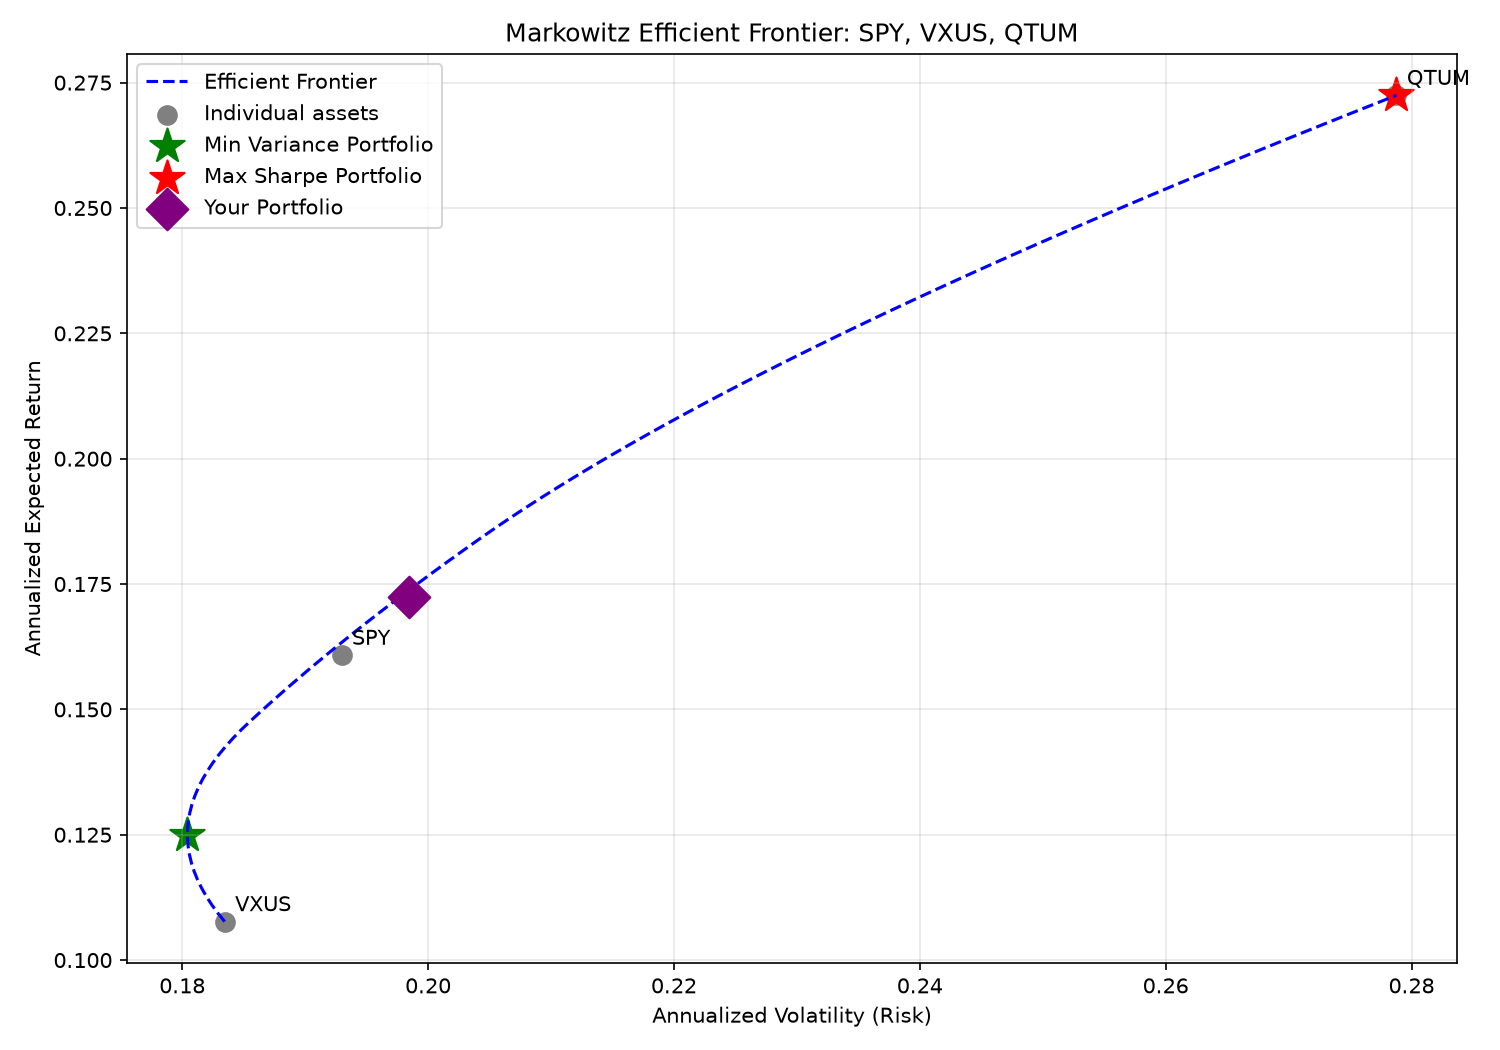
\includegraphics[width=0.85\textwidth]{figures/efficient_frontier.png}
\caption{Markowitz efficient frontier for SPY, VXUS, and QTUM, with the
minimum-variance portfolio, maximum-Sharpe portfolio, and a fixed 60/20/20
allocation marked.}
\label{fig:frontier}
\end{figure}

As the figure shows, the fixed 60/20/20 portfolio sits strictly inside the
frontier rather than on it -- it is, by construction, mean-variance
sub-optimal relative to what the unconstrained optimizer can achieve. It
nonetheless offers meaningfully more balanced exposure across all three
assets than either corner solution, at a risk and return profile between
the minimum-variance and maximum-Sharpe extremes.

\section{Conclusion and Implications}

The results illustrate a central practical tension in mean-variance
portfolio construction. Mathematically, the optimizer is doing exactly what
it is asked to do: for this three-asset universe and this particular sample
of historical returns, holding 100\% QTUM genuinely does maximize the
in-sample Sharpe ratio, and a SPY/VXUS blend genuinely does minimize
in-sample variance. But neither output resembles what most investors would
consider a diversified portfolio, and both are highly sensitive to the
specific sample window used to estimate $\boldsymbol{\mu}$ and $\Sigma$.
This sensitivity -- sometimes called ``error maximization'' in mean-variance
optimization \citep*{michaud1989} -- means that a small change in the
estimation window or the assumed risk-free rate can flip the optimal
portfolio from one corner to another.

A fixed, manually chosen allocation such as 60/20/20 avoids this fragility
by construction, at the cost of being provably sub-optimal against the
in-sample frontier. Whether that trade-off is worthwhile depends on how
much an investor trusts the sample estimates to hold out of sample -- and
for a three-asset universe with a highly volatile, high-return thematic
fund like QTUM, there is good reason for skepticism.

Natural extensions of this analysis include: (i) imposing a maximum
per-asset weight constraint so the optimizer is forced to diversify, (ii)
using a shrinkage estimator (e.g., Ledoit--Wolf) for the covariance matrix
to reduce estimation noise, (iii) applying a Black--Litterman framework to
blend the historical sample mean with an investor's own return views, and
(iv) evaluating all portfolios out-of-sample via a rolling or expanding
backtest rather than relying on a single in-sample estimation window.

\appendix

\section{Reproducing These Results}

The full analysis, including data download, optimization, and plotting
code, is available as a standalone Python package. The efficient frontier
in Figure~\ref{fig:frontier}, including the custom 60/20/20 marker, is
generated with:

\begin{lstlisting}[style=python, numbers=none]
python -m markowitz.cli --weights 0.6 0.2 0.2 --output-dir outputs/custom_60_20_20
\end{lstlisting}

\section{Core Optimization Code}

\begin{lstlisting}[style=python]
def portfolio_performance(weights, mean_returns, cov_matrix):
    """Return (expected_return, volatility) for a given weight vector."""
    ret = float(np.dot(weights, mean_returns))
    vol = float(np.sqrt(weights.T @ cov_matrix.values @ weights))
    return ret, vol


def min_variance_portfolio(mean_returns, cov_matrix, allow_short=False):
    """Solve for the global minimum-variance portfolio."""
    n = len(mean_returns)
    init = np.repeat(1 / n, n)
    constraints = ({"type": "eq", "fun": lambda w: np.sum(w) - 1},)
    bounds = tuple((-1.0, 1.0) if allow_short else (0.0, 1.0) for _ in range(n))
    result = minimize(
        lambda w, mu, cov: portfolio_performance(w, mu, cov)[1],
        init, args=(mean_returns, cov_matrix),
        method="SLSQP", bounds=bounds, constraints=constraints,
    )
    return result.x


def max_sharpe_portfolio(mean_returns, cov_matrix, risk_free_rate, allow_short=False):
    """Solve for the maximum Sharpe ratio (tangency) portfolio."""
    n = len(mean_returns)
    init = np.repeat(1 / n, n)

    def neg_sharpe(w, mu, cov, rf):
        ret, vol = portfolio_performance(w, mu, cov)
        return -(ret - rf) / vol

    constraints = ({"type": "eq", "fun": lambda w: np.sum(w) - 1},)
    bounds = tuple((-1.0, 1.0) if allow_short else (0.0, 1.0) for _ in range(n))
    result = minimize(
        neg_sharpe, init, args=(mean_returns, cov_matrix, risk_free_rate),
        method="SLSQP", bounds=bounds, constraints=constraints,
    )
    return result.x
\end{lstlisting}

Full source, including the CLI, plotting, and test suite, is available in
the accompanying \texttt{markowitz-portfolio-optimizer} repository.

\begin{thebibliography}{9}

\bibitem[Markowitz, 1952]{markowitz1952}
Markowitz, H. (1952). Portfolio Selection. \textit{The Journal of Finance},
7(1), 77--91.

\bibitem[Michaud, 1989]{michaud1989}
Michaud, R. O. (1989). The Markowitz Optimization Enigma: Is `Optimized'
Optimal? \textit{Financial Analysts Journal}, 45(1), 31--42.

\end{thebibliography}

\end{document}
